\subsection{Package \lstinline!cryptocast.util!}
Utility classes that are not specific to CryptoCast and don't fit any of the other packages.

\noindent\begin{minipage}[t]{5cm}
\vspace{0.3em}
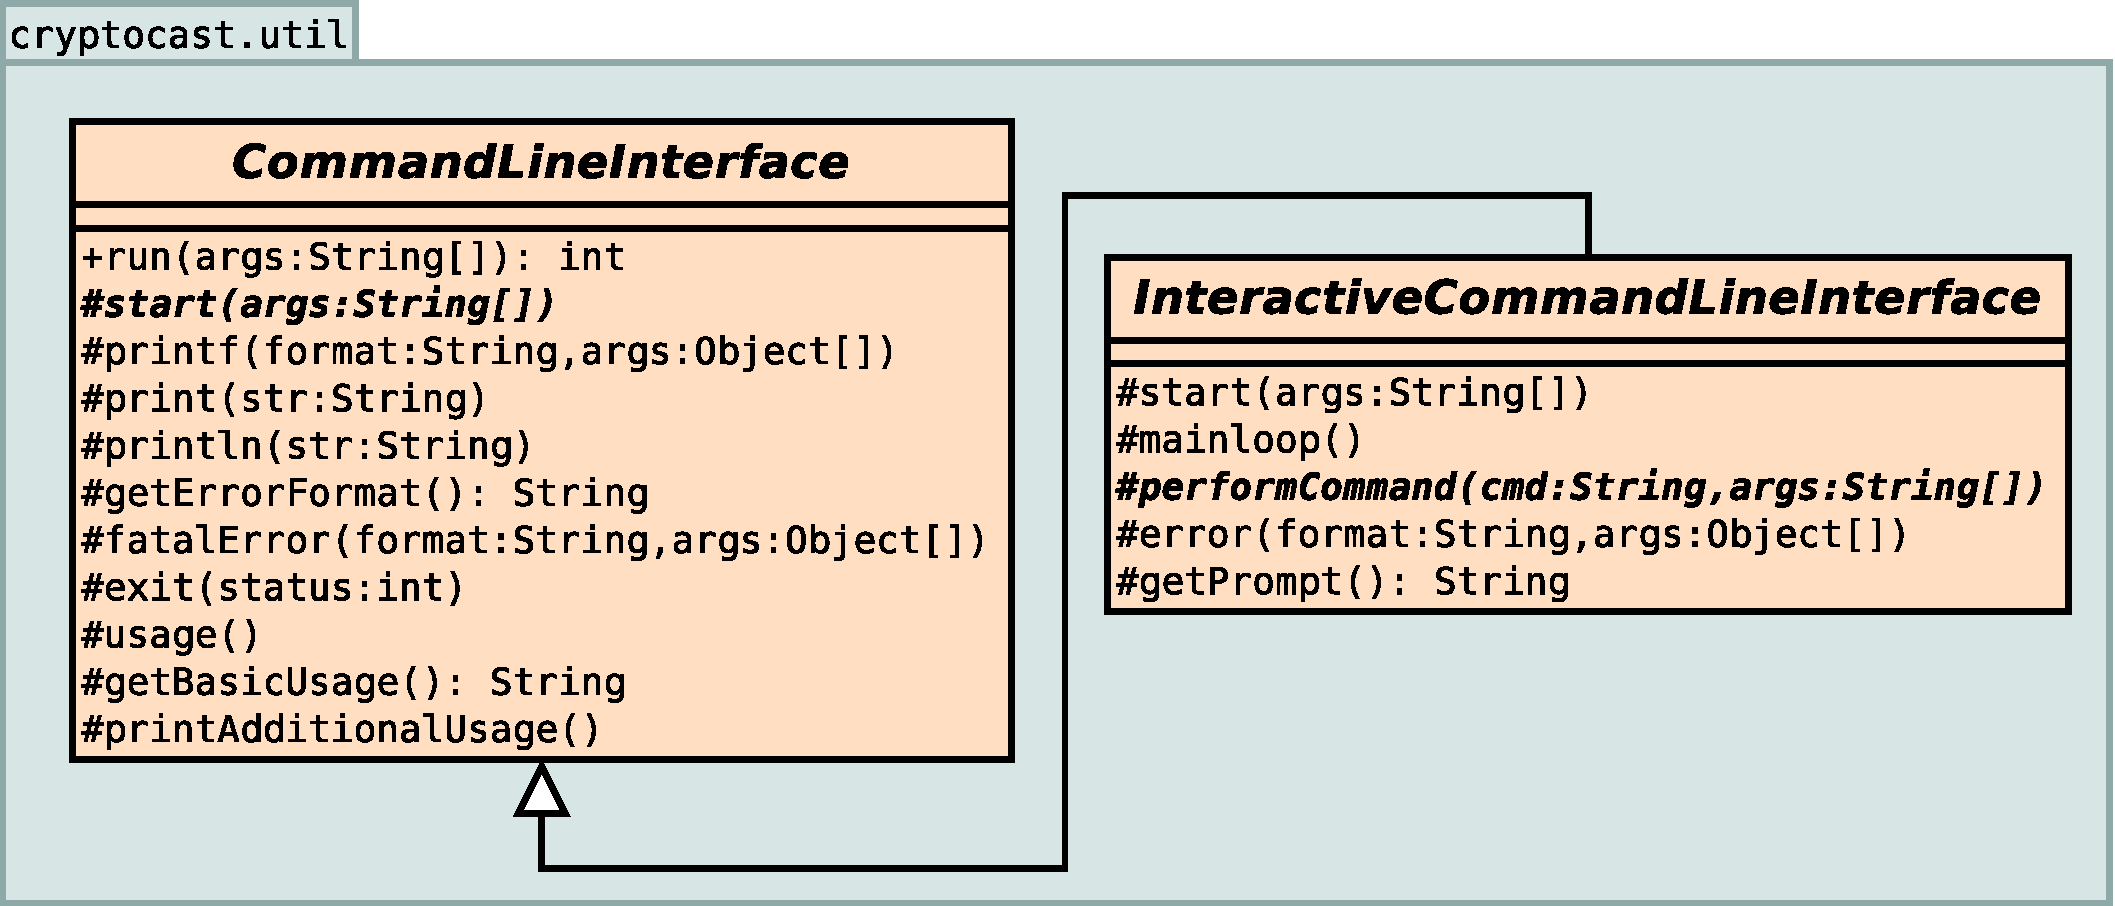
\includegraphics[width=300px]{class_diagrams/cryptocast_util.pdf}
\end{minipage}

\subsubsection{Class \lstinline|OptimisticGenerator<T>|}
An generator of a function $f: \mathbb{N} \to T$ that computes ranges in
 steps of powers of two. That way, we can make optimal use of a \lstinline|getRange|
 implementation that is more efficient if the range is large, while ensuring
 that we never compute more than twice as many values as we actually need.

 This instance also caches all the generated values, so that no value is
 computed twice. This makes it valid for the underlying generator to create
 random values and expected them to be saved. \\
\noindent\begin{minipage}[t]{5cm}
\vspace{0.3em}
\hspace*{2em}
\begin{tikzpicture}
\umlclass[]{OptimisticGenerator<T>}{

}{
+ get(i : int) : T \\
+ getRange(a : int, b : int) : ImmutableList<T>
}
\end{tikzpicture}
\vspace{0.3em}
\end{minipage}

\begin{itemize}
\item \lstinline|<T>|: the type of the generator object.
\end{itemize}


\textbf{\sffamily Superclasses and Interfaces}
\begin{itemize}
\item \lstinline|cryptocast.util.Generator<T>|
\item \lstinline|java.io.Serializable|
\end{itemize}


\textbf{\sffamily Constructors}
\begin{itemize}
\item \lstinline|public| \lstinline|OptimisticGenerator|\lstinline|(Generator<T> inner)|\\ \\[-0.6em]
Creates an instance of this class.
\begin{itemize}
\item \lstinline|inner|: The generator upon which this generator is based.
\end{itemize}



\end{itemize}


\textbf{\sffamily Methods}
\begin{itemize}
\item \lstinline|public T| \lstinline|get|\lstinline|(int i)| \\[-0.6em]




\item \lstinline|public ImmutableList<T>| \lstinline|getRange|\lstinline|(int a, int b)| \\[-0.6em]




\end{itemize}

\subsubsection{Class \lstinline|SerializationUtils|}
Provides several utility function for object serialization. \\
\noindent\begin{minipage}[t]{5cm}
\vspace{0.3em}
\hspace*{2em}
\begin{tikzpicture}
\umlclass[]{SerializationUtils}{

}{
\umlstatic{+ readFromStream(in : InputStream) : T} \\
\umlstatic{+ readFromFile(file : File) : T} \\
\umlstatic{+ writeToStream(out : OutputStream, obj : Serializable)} \\
\umlstatic{+ writeToFile(file : File, obj : Serializable)}
}
\end{tikzpicture}
\vspace{0.3em}
\end{minipage}





\textbf{\sffamily Methods}
\begin{itemize}
\item \lstinline|public static T| \lstinline|readFromStream|\lstinline|(InputStream in)|\\ \\[-0.6em]
Deserializes an object from a stream.
\begin{itemize}
\item \lstinline|in|: The stream to read from.
\end{itemize}

\emph{Returns:} An instance of T

\item \lstinline|public static T| \lstinline|readFromFile|\lstinline|(File file)|\\ \\[-0.6em]
Deserializes an object from a file.
\begin{itemize}
\item \lstinline|file|: The file to read from.
\end{itemize}

\emph{Returns:} An instance of T

\item \lstinline|public static void| \lstinline|writeToStream|\lstinline|(OutputStream out, Serializable obj)|\\ \\[-0.6em]
Serialize an object into an output stream.
\begin{itemize}
\item \lstinline|out|: The output stream.
\item \lstinline|obj|: The object to write.
\end{itemize}



\item \lstinline|public static void| \lstinline|writeToFile|\lstinline|(File file, Serializable obj)|\\ \\[-0.6em]
Serialize an object into a file.
\begin{itemize}
\item \lstinline|file|: The file to write in.
\item \lstinline|obj|: The object to write.
\end{itemize}



\end{itemize}

\subsubsection{Class \lstinline|ByteUtils|}
Several bytes and byte arrays utility funtions. \\
\noindent\begin{minipage}[t]{5cm}
\vspace{0.3em}
\hspace*{2em}
\begin{tikzpicture}
\umlclass[]{ByteUtils}{

}{
\umlstatic{+ str2bytes(str : String) : byte[]} \\
\umlstatic{+ encodeUtf8(str : String) : byte[]}
}
\end{tikzpicture}
\vspace{0.3em}
\end{minipage}





\textbf{\sffamily Methods}
\begin{itemize}
\item \lstinline|public static byte[]| \lstinline|str2bytes|\lstinline|(String str)|\\ \\[-0.6em]
Converts a string to byte array.
\begin{itemize}
\item \lstinline|str|: The string.
\end{itemize}

\emph{Returns:} A byte array.

\item \lstinline|public static byte[]| \lstinline|encodeUtf8|\lstinline|(String str)|\\ \\[-0.6em]
Encodes a string using UTF-8.
\begin{itemize}
\item \lstinline|str|: The string.
\end{itemize}

\emph{Returns:} A byte array representing the UTF-8 encoded string.

\end{itemize}

\subsubsection{Class \lstinline|CommandLineInterface|}
A simple framework for command line programs. \\
\noindent\begin{minipage}[t]{5cm}
\vspace{0.3em}
\hspace*{2em}
\begin{tikzpicture}
\umlclass[type=abstract]{CommandLineInterface}{

}{
+ run() : int
}
\end{tikzpicture}
\vspace{0.3em}
\end{minipage}




\textbf{\sffamily Constructors}
\begin{itemize}
\item \lstinline|public| \lstinline|CommandLineInterface|\lstinline|(BufferedReader in, PrintStream out, PrintStream err)|\\ \\[-0.6em]
Initializes a new CLI instance.
\begin{itemize}
\item \lstinline|in|: The stream for program input
\item \lstinline|out|: The stream for program output
\item \lstinline|err|: The stream for error output
\end{itemize}



\end{itemize}


\textbf{\sffamily Methods}
\begin{itemize}
\item \lstinline|public int| \lstinline|run|\lstinline|()|\\ \\[-0.6em]
Runs the application.

\emph{Returns:} The exit code

\end{itemize}

\subsubsection{Class \lstinline|CommandLineInterface.Exit|}
Signals the exit of the application. \\
\noindent\begin{minipage}[t]{5cm}
\vspace{0.3em}
\hspace*{2em}
\begin{tikzpicture}
\umlclass[]{CommandLineInterface.Exit}{

}{
+ getStatus() : int
}
\end{tikzpicture}
\vspace{0.3em}
\end{minipage}



\textbf{\sffamily Superclasses and Interfaces}
\begin{itemize}
\item \lstinline|java.lang.Throwable|
\end{itemize}


\textbf{\sffamily Constructors}
\begin{itemize}
\item \lstinline|public| \lstinline|CommandLineInterface.Exit|\lstinline|(int status)|\\ \\[-0.6em]
Initializes a new Exit instance.
\begin{itemize}
\item \lstinline|status|: The exit code
\end{itemize}



\end{itemize}


\textbf{\sffamily Methods}
\begin{itemize}
\item \lstinline|public int| \lstinline|getStatus|\lstinline|()|\\ \\[-0.6em]
\emph{Returns:} The exit code



\end{itemize}

\subsubsection{Class \lstinline|Generator<T>|}
An abstract entity that models a function over the intergers ($f: \mathbb{Z}
 \to T$) \\
\noindent\begin{minipage}[t]{5cm}
\vspace{0.3em}
\hspace*{2em}
\begin{tikzpicture}
\umlclass[type=abstract]{Generator<T>}{

}{
\umlvirt{+ get(i : int) : T} \\
+ getRange(a : int, b : int) : ImmutableList<T>
}
\end{tikzpicture}
\vspace{0.3em}
\end{minipage}

\begin{itemize}
\item \lstinline|<T>|: The object type for range generator.
\end{itemize}




\textbf{\sffamily Methods}
\begin{itemize}
\item \lstinline|public abstract T| \lstinline|get|\lstinline|(int i)|\\ \\[-0.6em]
\emph{Returns:} the value $f(i)$



\item \lstinline|public ImmutableList<T>| \lstinline|getRange|\lstinline|(int a, int b)|\\ \\[-0.6em]
Given an interval $[a, b)$ of integers, this functions will compute the
 values $(f(a), f(a + 1), ..., f(b - 1))$.
\begin{itemize}
\item \lstinline|a|: The left interval bound (inclusive).
\item \lstinline|b|: The right interval bound (exclusive).
\end{itemize}

\emph{Returns:} a \lstinline|List| of values representing the generated range.

\end{itemize}

\subsubsection{Class \lstinline|MapUtils|}
Provides map utility methods. \\
\noindent\begin{minipage}[t]{5cm}
\vspace{0.3em}
\hspace*{2em}
\begin{tikzpicture}
\umlclass[]{MapUtils}{

}{
\umlstatic{+ zip(keys : Iterable<T>, values : Iterable<U>) : ImmutableMap<T, U>}
}
\end{tikzpicture}
\vspace{0.3em}
\end{minipage}





\textbf{\sffamily Methods}
\begin{itemize}
\item \lstinline|public static ImmutableMap<T, U>| \lstinline|zip|\lstinline|(Iterable<T> keys, Iterable<U> values)|\\ \\[-0.6em]
Build a map with the given keys and values.
\begin{itemize}
\item \lstinline|keys|: The keys of the map.
\item \lstinline|values|: The values of the map.
\end{itemize}

\emph{Returns:} A map with the given keys and values.

\end{itemize}

\subsubsection{Class \lstinline|FileUtils|}
Provides utility methods for file paths. \\
\noindent\begin{minipage}[t]{5cm}
\vspace{0.3em}
\hspace*{2em}
\begin{tikzpicture}
\umlclass[]{FileUtils}{

}{
\umlstatic{+ expandPath(path : String) : File}
}
\end{tikzpicture}
\vspace{0.3em}
\end{minipage}





\textbf{\sffamily Methods}
\begin{itemize}
\item \lstinline|public static File| \lstinline|expandPath|\lstinline|(String path)|\\ \\[-0.6em]
Expands the given tilde-path (\lstinline|~/path/to/something|) into an absolute path.
\begin{itemize}
\item \lstinline|path|: The given path.
\end{itemize}

\emph{Returns:} The absolute path.

\end{itemize}

\subsubsection{Class \lstinline|InteractiveCommandLineInterface|}
A framework class to implement interactive command-line interfaces. The class implements
 a read-parse-execute main loop and provides hooks for subclasses to implement the missing
 functionality. \\
\noindent\begin{minipage}[t]{5cm}
\vspace{0.3em}
\hspace*{2em}
\begin{tikzpicture}
\umlclass[type=abstract]{InteractiveCommandLineInterface}{

}{

}
\end{tikzpicture}
\vspace{0.3em}
\end{minipage}



\textbf{\sffamily Superclasses and Interfaces}
\begin{itemize}
\item \lstinline|cryptocast.util.CommandLineInterface|
\end{itemize}


\textbf{\sffamily Constructors}
\begin{itemize}
\item \lstinline|public| \lstinline|InteractiveCommandLineInterface|\lstinline|(BufferedReader in, PrintStream out, PrintStream err)|\\ \\[-0.6em]
Initializes a new interactive CLI instance.
\begin{itemize}
\item \lstinline|in|: The stream for program input
\item \lstinline|out|: The stream for program output
\item \lstinline|err|: The stream for error output
\end{itemize}



\end{itemize}


\subsubsection{Class \lstinline|InteractiveCommandLineInterface.CommandError|}
An error within one of the commands. Will be caught by the main loop. \\
\noindent\begin{minipage}[t]{5cm}
\vspace{0.3em}
\hspace*{2em}
\begin{tikzpicture}
\umlclass[]{InteractiveCommandLineInterface.CommandError}{

}{
+ getMessage() : String
}
\end{tikzpicture}
\vspace{0.3em}
\end{minipage}



\textbf{\sffamily Superclasses and Interfaces}
\begin{itemize}
\item \lstinline|java.lang.Throwable|
\end{itemize}


\textbf{\sffamily Constructors}
\begin{itemize}
\item \lstinline|public| \lstinline|InteractiveCommandLineInterface.CommandError|\lstinline|(String msg)|\\ \\[-0.6em]
Initializes the error.
\begin{itemize}
\item \lstinline|msg|: The error message
\end{itemize}



\end{itemize}


\textbf{\sffamily Methods}
\begin{itemize}
\item \lstinline|public String| \lstinline|getMessage|\lstinline|()|\\ \\[-0.6em]
\emph{Returns:} The associated error message.



\end{itemize}

\subsubsection{Class \lstinline|ErrorUtils|}
Provides several error handing utility methods. \\
\noindent\begin{minipage}[t]{5cm}
\vspace{0.3em}
\hspace*{2em}
\begin{tikzpicture}
\umlclass[]{ErrorUtils}{

}{
\umlstatic{+ cannotHappen(e : Throwable)} \\
\umlstatic{+ cannotHappen()}
}
\end{tikzpicture}
\vspace{0.3em}
\end{minipage}





\textbf{\sffamily Methods}
\begin{itemize}
\item \lstinline|public static void| \lstinline|cannotHappen|\lstinline|(Throwable e)|\\ \\[-0.6em]
Throws an exception/error when an exception occurs which shouldn't have happened.
 We use this function to assert that an exception \lstinline|e| cannot happen by
 catching it and calling \lstinline|cannotHappen(e)|.
\begin{itemize}
\item \lstinline|e|: The exception that shouldn't have happened.
\end{itemize}



\item \lstinline|public static void| \lstinline|cannotHappen|\lstinline|()|\\ \\[-0.6em]
Throws an exception/error when reached. We use this to assert that
 a point of code cannot be reached.



\end{itemize}

\subsubsection{Class \lstinline|NativeUtils|}
Provides convenience methods for calling optional native components. \\
\noindent\begin{minipage}[t]{5cm}
\vspace{0.3em}
\hspace*{2em}
\begin{tikzpicture}
\umlclass[]{NativeUtils}{

}{
\umlstatic{+ bigIntListToTwoComplements(bigInts : List<BigInteger>) : byte[][]} \\
\umlstatic{+ twoComplementsToBigIntList(twoComplements : byte[][]) : ImmutableList<BigInteger>} \\
\umlstatic{+ tryToLoadNativeLibOrLogFailure(lib : String, log : Logger) : boolean}
}
\end{tikzpicture}
\vspace{0.3em}
\end{minipage}





\textbf{\sffamily Methods}
\begin{itemize}
\item \lstinline|public static byte[][]| \lstinline|bigIntListToTwoComplements|\lstinline|(List<BigInteger> bigInts)|\\ \\[-0.6em]
Converts a list of \lstinline|BigInteger| into their two-complements representation.
\begin{itemize}
\item \lstinline|bigInts|: The big integers.
\end{itemize}

\emph{Returns:} Their two-complements representations.

\item \lstinline|public static ImmutableList<BigInteger>| \lstinline|twoComplementsToBigIntList|\lstinline|(byte[][] twoComplements)|\\ \\[-0.6em]
Converts numbers given in their two-complements representation  into a list of
 \lstinline|BigInteger|s.
\begin{itemize}
\item \lstinline|twoComplements|: The two-complements.
\end{itemize}

\emph{Returns:} A list of big integers.

\item \lstinline|public static boolean| \lstinline|tryToLoadNativeLibOrLogFailure|\lstinline|(String lib, Logger log)|\\ \\[-0.6em]
Tries to load a native library, logs an error if loading failed.
\begin{itemize}
\item \lstinline|lib|: The library to load.
\item \lstinline|log|: The logger to log the error.
\end{itemize}

\emph{Returns:} \lstinline|true| if the library could be loaded, \lstinline|false| otherwise.

\end{itemize}

\subsubsection{Interface \lstinline|CanBeObserved|}
Describes a class that can be observed. Can be used instead of the \lstinline|Observable| base classes in cases where we can't use it because we inherit
 from a different class. \\
\noindent\begin{minipage}[t]{5cm}
\vspace{0.3em}
\hspace*{2em}
\begin{tikzpicture}
\umlclass[type=abstract]{CanBeObserved}{

}{
\umlvirt{+ addObserver(o : Observer)} \\
\umlvirt{+ deleteObserver(o : Observer)}
}
\end{tikzpicture}
\vspace{0.3em}
\end{minipage}





\textbf{\sffamily Methods}
\begin{itemize}
\item \lstinline|public void| \lstinline|addObserver|\lstinline|(Observer o)|\\ \\[-0.6em]
Adds an observer to the class.
\begin{itemize}
\item \lstinline|o|: The new observer
\end{itemize}



\item \lstinline|public void| \lstinline|deleteObserver|\lstinline|(Observer o)|\\ \\[-0.6em]
Removes an observer from the class.
\begin{itemize}
\item \lstinline|o|: The old observer
\end{itemize}



\end{itemize}


